\section{Related Work}
\label{sec:related_work}

We view model-based safety analysis as an extension of model-based systems engineering. Our 
goal is to extend an existing system model to add information needed for safety analysis.
Model-based safety analysis approaches have been developed for a variety of modeling languages, 
including SysML~\cite{friedenthal2014practical, helle2012automatic,mhenni2014automatic}, AADL~\cite{AADL_Standard, EMV2}, SLIM~\cite{10.1007/978-3-642-04468-7_15}, Simulink~\cite{MathWorks, Joshi05:SafeComp}, and others. 
Each language has a targeted domain of application and contains different levels of formalism.
For example, SysML is normally used to describe graphical system model in the early stages of 
development to explore requirement, use cases, and design trade-offs, while AADL provides a 
more rigorous system description and run-time semantics that better supports analysis and 
implementation.  Due to the formal model checking approach we have used in the safety annex, 
we chose to extend a modeling language with well-defined semantics with a focus on modeling 
real-time embedded systems.

A model-based approach for safety analysis was proposed by Joshi et. al in \cite{Joshi05:Dasc, Joshi05:SafeComp, Joshi07:Hase}.  In this approach, a \gls{sasm} is the central artifact in the safety analysis process, and traditional safety analysis artifacts, such as fault trees, are automatically generated by tools that analyze the SASM.

The contents and structure of the \gls{sasm} differ significantly across different conceptions of \gls{mbsa}.  We can draw distinctions between approaches along several different axes.  The first is whether they propagate faults explicitly through user-defined propagations, which we call \gls{flm} or through existing behavioral modeling, which we call \gls{fem}.  The next is whether models and notations are {\em purpose-built} for safety analysis vs. those that extend {\em existing system models} (ESM).

For \gls{fem} approaches, there are several additional dimensions.  One dimension involves whether {\em causal} or {\em non-causal} models are allowed.  Non-causal models allow simultaneous (in time) bi-directional %failure
error propagations, which allow more natural expression of some failure types (e.g. reverse flow within segments of a pipe), but are more difficult to analyze.  A final dimension involves whether analysis is {\em compositional} across layers of hierarchically-composed systems or {\em monolithic}.  Our approach is an extension of \gls{aadl} (\gls{esm}), causal, compositional, mixed \gls{flm}/\gls{fem} approach.

Tools such as the \gls{aadl} Error Model Annex, Version 2 (EMV2)~\cite{EMV2}, HiP-HOPS for EAST-ADL~\cite{CHEN201391}, and Ansys Medini~\cite{ansys} are {\em \gls{flm}}-based {\em \gls{esm}} approaches.  As previously discussed, given many possible faults, these propagation relationships require substantial user effort and become more complex.  In addition, it becomes the analyst's responsibility to determine whether faults can propagate; missing propagations lead to unsound analyses.  In the safety annex, propagations occur through system behaviors (defined by the nominal contracts) with no additional user effort.

\begin{figure}[h!]
	\begin{centering}
		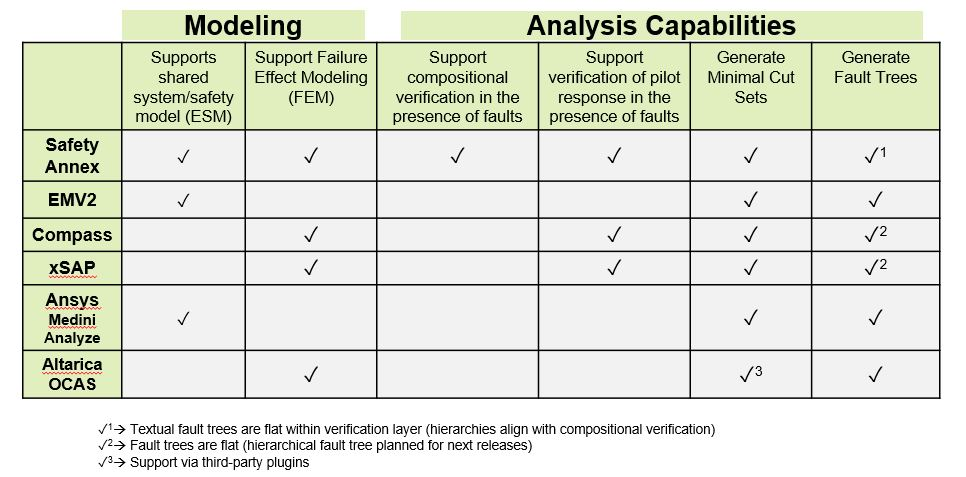
\includegraphics[width=\textwidth]{images/relatedwork.jpg}
		\caption{Related MBSA Tools and Methods}
		\label{fig:related}
	\end{centering}
\end{figure}

Figure~\ref{fig:related} shows a reference table listing a few of the related work tools we describe in the remainder of this section. The figure highlights important features of the support provided. Closely related to our work is the model-based safety assessment toolset called COMPASS (Correctness, Modeling project and Performance of Aerospace Systems)~\cite{10.1007/978-3-642-04468-7_15}.  COMPASS is a mixed {\em \gls{flm}/\gls{fem}}-based, {\em causal} tool suite that uses the SLIM language, which is based on a subset of AADL, for its input models~\cite{5185388, criticalembeddedsystems}. In SLIM, a nominal system model and the error model are developed separately and then transformed into an extended system model.  This extended model is automatically translated into input models for the NuSMV model checker~\cite{Cimatti2000, NuSMV}, MRMC (Markov Reward Model Checker)~\cite{Katoen:2005:MRM:1114692.1115230, MRMC}, and RAT (Requirements Analysis Tool)~\cite{RAT}. The safety analysis tool xSAP~\cite{DBLP:conf/tacas/BittnerBCCGGMMZ16} can be invoked in order to generate safety analysis artifacts such as fault trees and FMEA tables~\cite{compass30toolset}.  COMPASS is an impressive tool suite, but some of the features that make AADL suitable for SW/HW architecture specification: event and event-data ports, threads, and processes, appear to be missing, which means that the SLIM language may not be suitable as a general system design notation (\gls{esm}).

SmartIFlow~\cite{info17:HaLuHo} is a {\em \gls{fem}}-based, {\em purpose-built}, {\em monolithic} {\em non-causal} safety analysis tool that describes components and their interactions using finite state machines and events. Verification is done through an explicit state model checker which returns sets of counterexamples for safety requirements in the presence of failures.  SmartIFlow allows {\em non-causal} models containing simultaneous (in time) bi-directional %failure
error propagations.  On the other hand, the tools do not yet appear to scale to industrial-sized problems, as mentioned by the authors~\cite{info17:HaLuHo}: ``As current experience is based on models with limited size, there is still a long way to go to make this approach ready for application in an industrial context.''

The Safety Analysis and Modeling Language (SAML)~\cite{Gudemann:2010:FQQ:1909626.1909813} is a {\em FEM}-based, {\em purpose-built}, {\em monolithic} {\em causal} safety analysis language.  System models constructed in SAML can be used for both qualitative and quantitative analyses. It allows for the combination of discrete probability distributions and non-determinism. The SAML model can be automatically imported into several analysis tools like NuSMV~\cite{Cimatti2000}, PRISM (Probabilistic Symbolic Model Checker)~\cite{CAV2011:KwNoPa}, or the MRMC probabilistic model checker~\cite{Katoen:2005:MRM:1114692.1115230}. 

AltaRica~\cite{PROSVIRNOVA2013127,BieberERTS2018} is a {\em \gls{fem}}-based, {\em purpose-built}, {\em monolithic} safety analysis language with several dialects.  There is one dialect of AltaRica which uses dataflow ({\em causal}) semantics, while the most recent language update (AltaRica 3.0) uses non-causal semantics.  The dataflow dialect has substantial tool support, including the commercial Cecilia OCAS tool from Dassault~\cite{Bieber04safetyassessment}.  For this dialect the Safety assessment, fault tree generation, and functional verification can be performed with the aid of NuSMV model checking~\cite{symbAltaRica}. Failure states are defined throughout the system and flow variables are updated through the use of assertions~\cite{BieberERTS2018}.  AltaRica 3.0 has support for simulation and Markov model generation through the OpenAltaRica (www.openaltarica.fr) tool suite.

Formal verification tools based on model checking have been used to automate the generation of safety artifacts~\cite{symbAltaRica,10.1007/978-3-540-75596-8-13, DBLP:conf/tacas/BittnerBCCGGMMZ16}. This approach has limitations in terms of scalability and readability of the fault trees generated. Work has been done towards mitigating these limitations by the scalable generation of readable fault trees~\cite{10.1007/978-3-319-11936-6-7}.




